\documentclass[12]{beamer}
\usefonttheme[onlymath]{serif}
\usepackage{amsmath}
\usetheme{CambridgeUS}
\setbeamertemplate{enumerate items}[default]

% \setbeamercolor*{enumerate item}{fg=brown}

\begin{document}

%
% parametric methods
%

\begin{frame}
  \frametitle{Parametric Methods}
  \begin{itemize}
	\addtolength{\itemsep}{5pt}
	\item Reduce the problem of estimating f down to one of estimating a set of \textit{parameters}
	\item Involve a two-step model-based approach
	\begin{enumerate}
	  	\item First, we make an assumption about the functional form, or shape, of \textbf{\textit{f}}. For example, one very simple assumption is that f is linear in $X$:
	  	\begin{equation} \label{eq:1}
	  	  f(x) = \beta_{0} + \beta_{1}X_{1} + \beta_{2}X_{2} + ... + \beta_{p}X_{p}
	  	\end{equation}
	  	Once it is assumed that f follows a certain shape (linear in the above example), the p+1 coefficients need to be estimated.
	  	
	  	\item After a model has been selected, a procedure to train the model using the training data is selected. The most common
	  	approach to fitting linear models is \textit(ordinary) least squares. However, \textit{least squares} is just one of many possible
	  	ways to fit a linear model.
	\end{enumerate}
  \end{itemize}
\end{frame}

\begin{frame}
  \frametitle{Parametric Methods }
  \begin{itemize}
    \addtolength{\itemsep}{5pt}
    \item Assuming a parametric form for f simplifies the estimation of f as it is generally much easier to estimate a set of parameters,
    such as $\beta_{0}, \beta_{1}, ...., \beta_{p}$ in the linear model than it is to fit an entirely arbitrary function.
    \item The potential disadvantage of a parametric approach is that the chosen model will not usually match the true unknown form
    of f
    \item The above problem of a poor model can be addressed by choosing flexible models that can fit many different functional forms
    for f. However, fitting a more flexible model requires the estimation of a greater number of parameters.
    \item More complex models can lead to a phenomenon known as \textit{overfitting} the data, as they follow the errors or noise too
    closely.
  \end{itemize}
\end{frame}

%
% non-parametric methods
%
\begin{frame}
\frametitle{Non-Parametric Methods}
\begin{itemize}
\addtolength{\itemsep}{10pt}
\item Do not make explicit assumptions about the functional form of \textit{f}
\item Seek an estimate of f that gets as close to the data points as possible without being too wiggly and rough
\item Have the potential to accurately fit a wider range of possible shapes for f, by avoiding the assumption of a particular functional form
\item However, since they do not reduce the problem of estimating f to a small number of parameters, a very large number of observations (far more than is typically needed for a parametric approach) is required in order to obtain an accurate estimate for \textit{\textbf{f}}
\end{itemize}
\end{frame}

%
% Variance
%
\begin{frame}
\frametitle{Variance}
\begin{itemize}
\addtolength{\itemsep}{10pt}
\item Refers to the amount by which $\hat{f}$ would change if we estimated it using a different training data set
\item Since the training data are used to fit the statistical learning method, different training data sets will result in a different $\hat{f}$
\item Ideally the estimate for f should not vary too much between training sets. However, if a method has high variance then small changes in the training data can result in large changes in $\hat{f}$
\item In general, more flexible statistical methods have higher variance as they follow the training set more closely
\end{itemize}
\end{frame}

%
% bias
%
\begin{frame}
\frametitle{Bias}
\begin{itemize}
\addtolength{\itemsep}{10pt}
\item Refers to the error that is introduced by approximating a real-life problem, which may be extremely complicated, by a much
simpler model.
\item For example, linear regression assumes that there is a linear relationship between $Y$ and $X_{1}, X_{2}, . . . , X_{p}$. It is unlikely that any real-life problem truly has such a simple linear relationship, and so performing linear regression will undoubtedly result in some bias in the estimate of \textit{\textbf{f}}
\item Generally, more flexible methods (with more degrees of freedom) result in less bias.
\end{itemize}
\end{frame}

%
% bias-variance tradeoff
%
\begin{frame}
  \frametitle{Bias-Variance Trade-Off}
  The expected test MSE, for a given value $x_{0}$, can always be decomposed into the sum of three fundamental quantities: the \textit{variance} of $\hat{f}(x_{0})$, the squared \textit{bias} of $\hat{f}(x_{0})$ and the variance of the error terms $\epsilon$.
\end{frame}

\begin{frame}
  \frametitle{figure test}
  \begin{figure}[hbt!]
  % \centering
  % 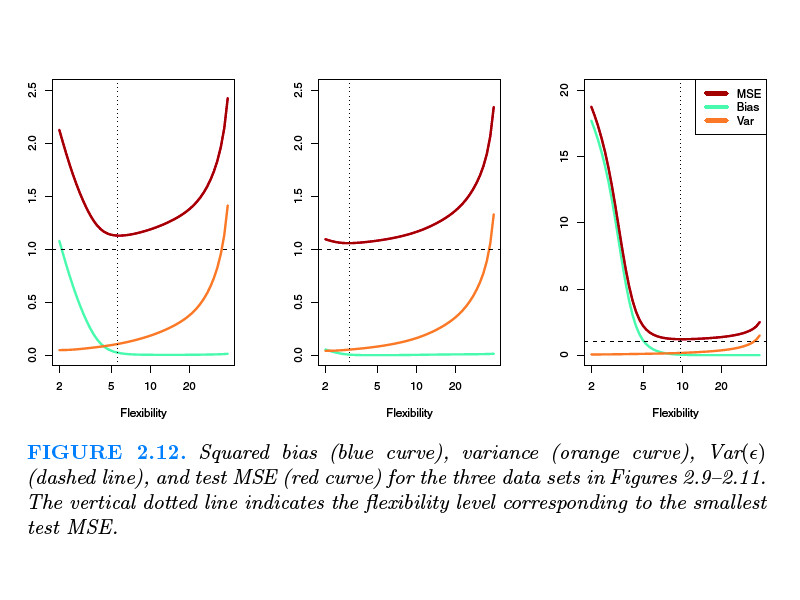
\includegraphics[scale=1.5,width=\linewidth,height=\textheight,keepaspectratio]{Untitled.jpg}
  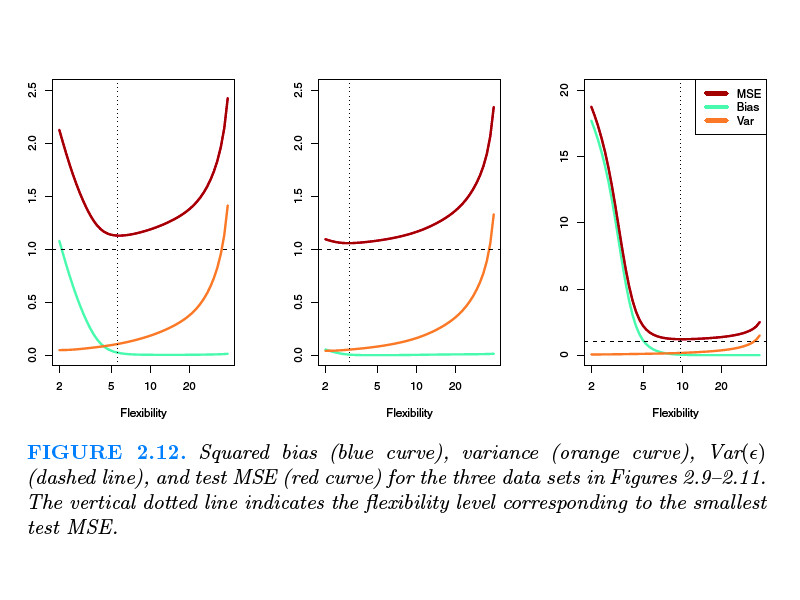
\includegraphics[scale=2.0,height=0.5\paperwidth,keepaspectratio]{Untitled.jpg}
  \end{figure}
\end{frame}

\begin{frame}
  \frametitle{The Classification Setting}
  \begin{itemize}
  	\addtolength{\itemsep}{5pt}
    \item we seek to estimate $f$ on the basis of training observations
          \{$(x_{1}, y_{1}), . . . , (x_{n}, y_{n})$\}, where now $y_{1}, . . . , y_{n}$ are qualitative
    \item The most common approach for quantifying the accuracy of our estimate $\hat{f}$ is the
          training error rate, the proportion of mistakes that are made if we apply error rate our
          estimate $\hat{f}$ to the training observations:
          \begin{equation}
            \color{blue}      
	  	    \displaystyle \frac{1}{n} \sum_{i=1}^{n} I(y_{i} \neq \hat{y_{i}})
	  	  \end{equation}
	  	  Here $\hat{y_{i}}$ is the predicted class label for the \textit{i}th observation using $\hat{f}$. And
	  	  $I(y_{i} \neq \hat{y_{i}})$ is an indicator variable that equals 1 if $y_{i} \neq \hat{y_{i}}$
	  	  and zero if $y_{i} = \hat{y_{i}}$.
  \end{itemize}
\end{frame}

\end{document}